\documentclass[11pt,letterpaper]{article}
\usepackage[T1]{fontenc}
\usepackage{lmodern,microtype,amsmath,amssymb,graphicx,booktabs,tabularx,array,enumitem,xcolor,fancyhdr,titlesec,tcolorbox,caption}
\tcbuselibrary{breakable}
\usepackage[margin=.8in,headheight=15pt,headsep=18pt,footskip=25pt]{geometry}
\usepackage[colorlinks=true,urlcolor=teal,linkcolor=olive]{hyperref}
\definecolor{olive}{HTML}{536240}\definecolor{ink}{HTML}{293329}\definecolor{teal}{HTML}{17677A}\definecolor{gold}{HTML}{A55C21}\definecolor{soft}{HTML}{EEF3E8}\definecolor{warm}{HTML}{FBEFDF}
\color{ink}\setlength{\parindent}{0pt}\setlength{\parskip}{7pt}
\setlist{leftmargin=1.4em,itemsep=3pt,topsep=3pt}
\renewcommand{\thesection}{10.\arabic{section}}
\titleformat{\section}{\Large\bfseries\color{olive}}{\thesection}{.6em}{}
\titleformat{\subsection}{\large\bfseries\color{teal}}{}{0pt}{}
\titlespacing*{\section}{0pt}{4pt}{12pt}\titlespacing*{\subsection}{0pt}{11pt}{4pt}
\pagestyle{fancy}\fancyhf{}\fancyhead[L]{\small\sffamily MATH\& 107 / WEEK 10}\fancyhead[R]{\small\sffamily Complexity and Prediction}\fancyfoot[L]{\small\sffamily Math in Society / Dr Lee}\fancyfoot[R]{\small\sffamily\thepage}\renewcommand{\headrulewidth}{.3pt}
\tcbset{boxrule=.5pt,arc=2mm,left=10pt,right=10pt,top=7pt,bottom=7pt,before skip=9pt,after skip=9pt,colframe=olive!35,colback=soft,fonttitle=\bfseries,coltitle=teal,colbacktitle=soft}
\newcolumntype{Y}{>{\raggedright\arraybackslash}X}
\captionsetup{font=small,labelformat=empty,textfont={color=teal},skip=7pt}
\hypersetup{pdftitle={Week 10: Complexity and the Limits of Prediction},pdfauthor={MATH and 107 / Dr Lee}}
\begin{document}
{\small\sffamily\color{olive}CHAPTER 10 / COMPLEXITY AND THE LIMITS OF PREDICTION\par}
\vspace{8pt}
{\fontsize{31}{35}\selectfont\bfseries\color{olive}Simple rules.\\Surprising worlds.\par}
\vspace{8pt}
{\large Follow a number through a maze, build a curve that keeps getting longer, and discover why an exact rule can still leave a forecast uncertain.\par}

A short instruction can produce an unexpectedly long journey, an intricate shape, or a trajectory that is difficult to forecast. Those are different kinds of complexity. This chapter develops them through calculations you can see and check.

\begin{center}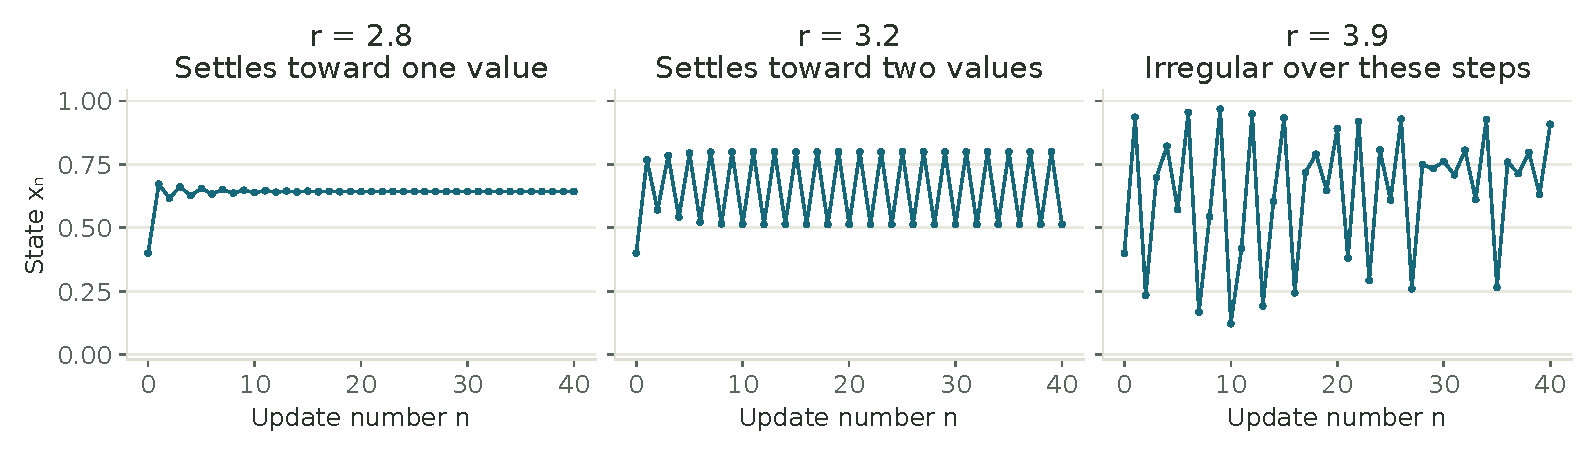
\includegraphics[width=\linewidth]{../assets/week10/logistic-behaviors.pdf}\end{center}
{\small\color{teal}The same logistic formula, starting from 0.4, produces different behavior when its parameter changes. The horizontal axis counts updates; the vertical axis records the state.\par}

\begin{tcolorbox}[title={The question for the week}]
If we know the rule, do we know the future? Identify three things: the update rule, the starting information, and the kind of conclusion we need.
\end{tcolorbox}
By the end of this chapter, you can trace Collatz routes, distinguish tested examples from proof, calculate fractal counts and measures, compare logistic forecasts, and report a measurement together with its observation scale.

Read the sections in order and attempt each ``Pause and try'' before checking the solutions at the end. The online explorer supplies numerical tables and tools for longer calculations. The starting value of a sequence always has index 0.

\medskip
\href{https://bobovski66.github.io/MathInSociety/readings/week10_reading.html}{Online reading}\quad\textperiodcentered\quad\href{https://bobovski66.github.io/MathInSociety/demos/fractal_recursion.html}{Week 10 explorer}\quad\textperiodcentered\quad\href{https://bobovski66.github.io/MathInSociety/labs/week10_lab.html}{Guided laboratory}

\clearpage

\section{One rule, many updates}

A \emph{recursion} uses a current value to calculate the next value. A \emph{trajectory} is the sequence of values it produces. The starting value has index 0; the result after one update has index 1.

\(\text{starting value }a_0 \quad\longrightarrow\quad a_1\quad\longrightarrow\quad a_2\quad\longrightarrow\cdots\)
\begin{tcolorbox}[title={Example 1 \textperiodcentered{} Read the subscript as a step counter},breakable]

Start with \(a_0=10\) and apply \(a_{n+1}=a_n+5\). The values are \(10,15,20,25,30,35\). The value after five updates is \(a_5=35\). There are \emph{six recorded values}, including the start.


\end{tcolorbox}

\subsection*{Compare two nearby starts}

``The difference gets bigger'' does not yet tell us what kind of behavior we have. We need to say which difference we mean.

\(\text{absolute difference}=|b_n-a_n|\qquad \text{relative difference}=\dfrac{|b_n-a_n|}{|a_n|}\)
The relative difference above uses the first trajectory as its reference and requires \(a_n\ne0\). Multiply by 100 to express it as a percentage.



{\small\renewcommand{\arraystretch}{1.35}\begin{tabularx}{\linewidth}{@{}YYY@{}}\toprule
Rule and starts & After the updates & What happened?\\
\midrule
Add 5; start at 10 and 10.1 & After 5 updates: 35 and 35.1 & Absolute gap stays 0.1.\\
Multiply by 3; start at 1 and 1.01 & After 6 updates: 729 and 736.29 & Gap is 7.29, but relative gap stays 1\%.\\
Multiply by 0.5; start at 10 and 10.1 & After 5 updates: 0.3125 and 0.315625 & Absolute gap shrinks to 0.003125.\\
\bottomrule\end{tabularx}}


\begin{tcolorbox}[title={Growing apart does not automatically mean chaos},breakable,colback=warm,colbacktitle=warm,coltitle=gold,colframe=gold!35]

In the multiplication example, both values grow by the same factor, so the gap is exactly predictable: \(0.01\cdot3^n\). A large absolute gap alone is not enough to identify chaotic behavior.


\end{tcolorbox}


\begin{tcolorbox}[title={Pause and try 1},breakable]
Start at 4 and 4.1. Double both values three times. What are the absolute and relative differences?
\end{tcolorbox}


\clearpage

\section{Two instructions. One enormous question.}

Choose a positive whole number. If it is even, divide it by 2. If it is odd, multiply it by 3 and add 1. Use the result as the next input.

\[a_{n+1}=\begin{cases}a_n/2,&a_n\text{ is even},\\3a_n+1,&a_n\text{ is odd}.\end{cases}\]

\begin{figure}[!htbp]
\centering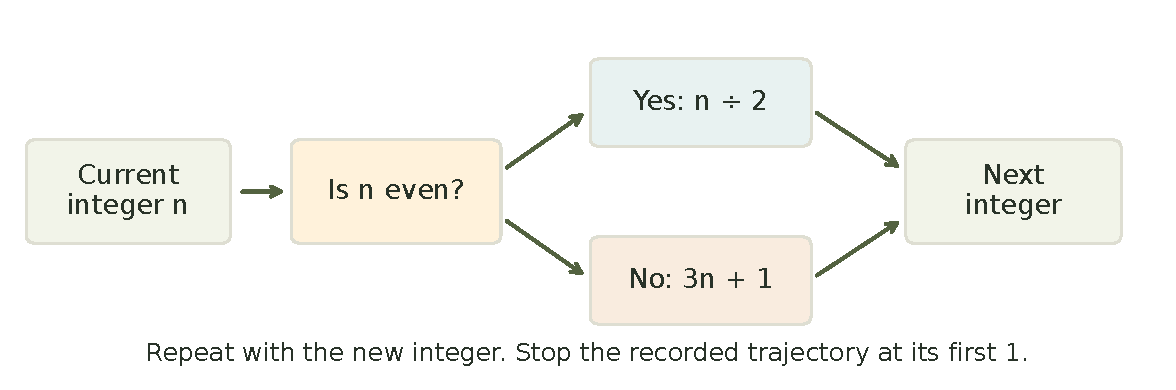
\includegraphics[width=.9\linewidth]{../assets/week10/collatz-rule.pdf}
\caption*{The parity test chooses the branch. No coin is tossed; each next value is determined by the current integer.}
\end{figure}


\begin{tcolorbox}[title={Example 2 \textperiodcentered{} Trace the route from 6},breakable]

First, 6 is even, so \(6/2=3\). Then 3 is odd, so \(3(3)+1=10\). Continue by checking the \emph{new} value each time.


\[6\to3\to10\to5\to16\to8\to4\to2\to1.\]

There are 8 arrows, so the trajectory first reaches 1 after \emph{8 updates}. Its largest value, or \emph{peak}, is 16. If we continue after 1, we get the repeating cycle \(1\to4\to2\to1\).


\end{tcolorbox}

\subsection*{Nearby starts can take very different routes}


{\small\renewcommand{\arraystretch}{1.35}\begin{tabularx}{\linewidth}{@{}YYY@{}}\toprule
Start & Updates to first 1 & Peak\\
\midrule
6 & 8 & 16\\
7 & 16 & 52\\
26 & 10 & 40\\
27 & 111 & 9,232\\
\bottomrule\end{tabularx}}


``Larger start'' does not reliably mean ``longer journey.'' For example, 32 reaches 1 in just five updates because \(32\to16\to8\to4\to2\to1\). The explorer lets you trace an entire route and compare neighboring starts.


\paragraph{A network connection.} Each integer has an arrow to its next value. Once two routes meet, their remaining routes agree exactly. The routes from 6 and 7 both reach 10.







\clearpage
\subsection*{Compare the journeys, then state the claim}
\begin{figure}[!htbp]
\centering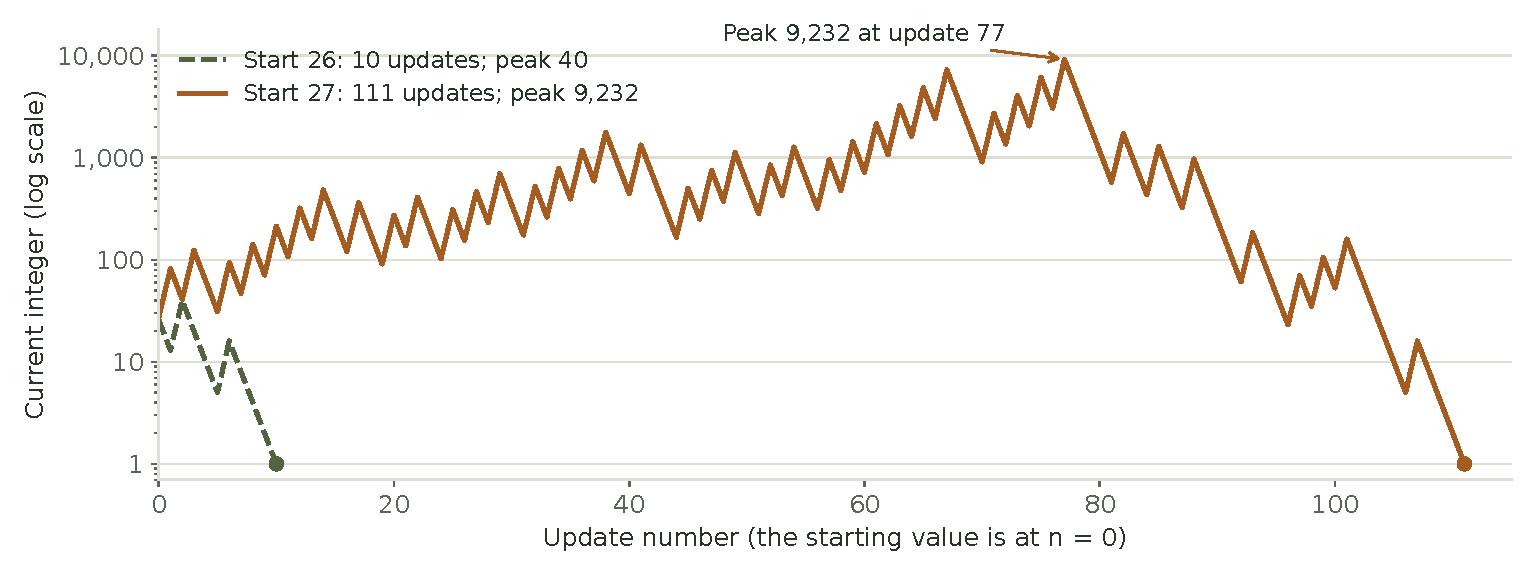
\includegraphics[width=\linewidth]{../assets/week10/collatz-comparison.pdf}
\caption*{Read the horizontal axis as an update count. On the logarithmic vertical axis, equal spacing represents multiplication by 10, so both the short and the tall trajectory remain visible.}
\end{figure}
\section{A million successful trials still leave a question}

The \emph{Collatz conjecture} says that every positive integer eventually reaches 1. Extensive computer searches support the conjecture, but a proof for every positive integer is still unknown. The exact rule is easy to state; the universal claim is difficult to establish.


\begin{tcolorbox}[title={Example 3 \textperiodcentered{} A family we really can prove},breakable]

If the starting number is a power of 2, say \(2^k\), each even step halves it:

\[2^k\to2^{k-1}\to\cdots\to2\to1.\]
It reaches 1 after exactly \(k\) updates. This argument works for \emph{every} nonnegative integer \(k\), so it covers infinitely many starts. It does not cover all positive integers: 7 and 27, for example, are not powers of 2.


\end{tcolorbox}

A finite computation can settle a stated finite range. A universal proof must explain why no positive integer outside that range can escape. Conversely, a single positive integer proved never to reach 1 would refute the conjecture.


\begin{tcolorbox}[title={Do not confuse two kinds of difficulty},breakable,colback=warm,colbacktitle=warm,coltitle=gold,colframe=gold!35]

Collatz gives surprising integer trajectories and an unresolved mathematical question. Comparing 26 and 27 does not establish chaos in the usual continuous-state sense. Later, the logistic map will give us a different question: what happens to an \emph{approximate measurement} under repeated updates?


\end{tcolorbox}


\begin{tcolorbox}[title={Pause and try 2},breakable]
A program tests every starting integer from 1 through 10,000, and they all reach 1. Which statement is justified?
\end{tcolorbox}





\clearpage
\section{Keep the rule. Change the scale.}

A self-similar object contains smaller copies of its overall pattern. We can build ideal fractals by repeating a geometric instruction at finer and finer scales. A displayed stage is a finite approximation; the ideal fractal is the limit of all stages.


\subsection*{The Koch curve: more pieces, longer total}

\begin{enumerate}
\item Begin with a straight segment of length 1.
\item Divide it into thirds. Replace the middle third with the two sides of an equilateral triangular bump.
\item Apply that replacement to \emph{every} segment of the new curve.

\end{enumerate}


\begin{figure}[!htbp]
\centering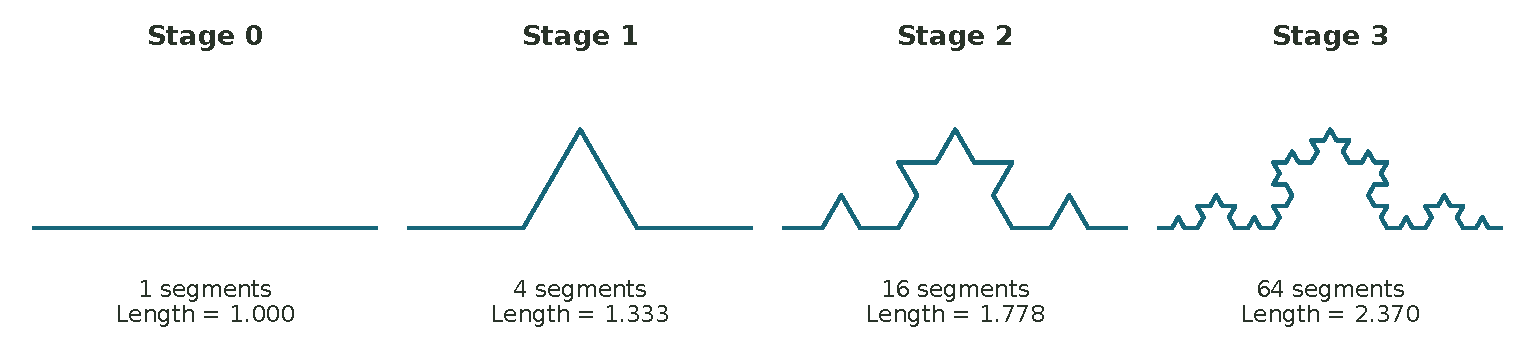
\includegraphics[width=\linewidth]{../assets/week10/koch-stages.pdf}
\caption*{The endpoints stay the same distance apart. The route between them gets longer because each old segment becomes four segments, each one-third as long.}
\end{figure}

\[N_n=4^n,\qquad \ell_n=\left(\frac13\right)^n,\qquad L_n=N_n\ell_n=\left(\frac43\right)^n.\]

{\small\renewcommand{\arraystretch}{1.35}\begin{tabularx}{\linewidth}{@{}YYYY@{}}\toprule
Stage n & Segment count N$_n$ & Length per segment $\ell$$_n$ & Total length L$_n$\\
\midrule
0 & 1 & 1 & 1\\
1 & 4 & 1/3 & 4/3 $\approx$ 1.3333\\
2 & 16 & 1/9 & 16/9 $\approx$ 1.7778\\
3 & 64 & 1/27 & 64/27 $\approx$ 2.3704\\
4 & 256 & 1/81 & 256/81 $\approx$ 3.1605\\
\bottomrule\end{tabularx}}


\begin{tcolorbox}[title={Example 4 \textperiodcentered{} A 9-meter starting segment},breakable]

After one replacement there are four 3-meter segments, totaling 12 meters. After two replacements there are sixteen 1-meter segments, totaling 16 meters.


Using the formula gives the same result: \(L_2=9(4/3)^2=16\) meters. The formula \((4/3)^n\) by itself assumes the original length is 1.


\end{tcolorbox}

\subsection*{The Sierpinski triangle: more pieces, less area}

Start with a filled triangle of area 1. Split it into four congruent triangles and remove the central one. Repeat on each remaining filled triangle. Each step keeps three quarters of the currently filled area.



\begin{figure}[!htbp]
\centering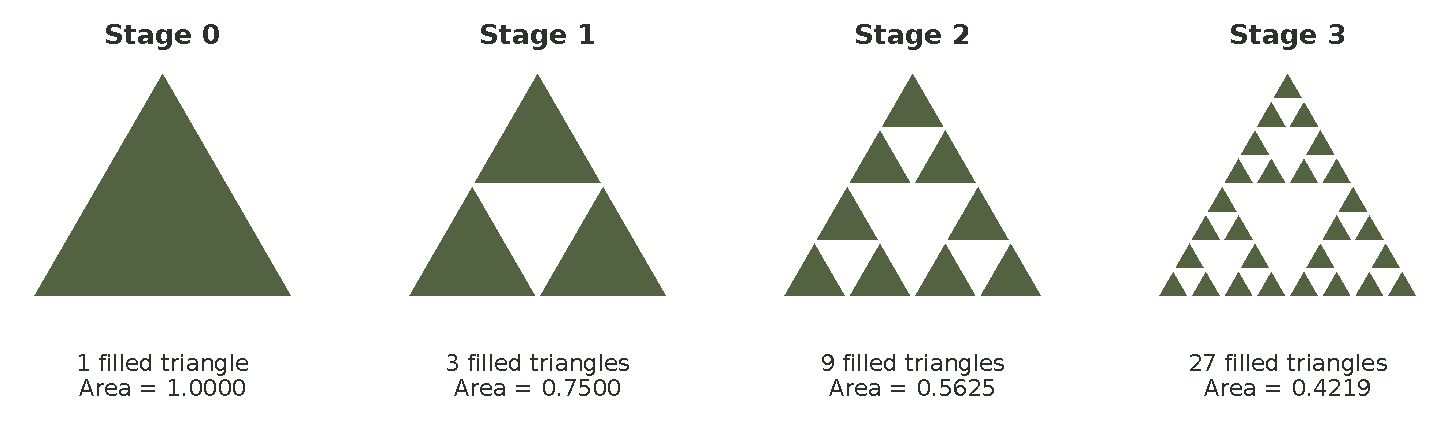
\includegraphics[width=\linewidth]{../assets/week10/sierpinski-stages.pdf}
\caption*{The number of pieces multiplies by 3, but each piece has one-quarter the area of its parent. Count and area answer different questions.}
\end{figure}

\[T_n=3^n,\qquad A_n=\left(\frac34\right)^n.\]
At stage 4, there are \(3^4=81\) filled triangles, yet only \((3/4)^4=81/256\approx0.3164\) of the original area remains. That is about 31.64\%, not 0.3164\%. In the ideal limit, the remaining area tends to zero while a rich self-similar set remains.


\begin{tcolorbox}[title={Geometric complexity can be exactly predictable},breakable,colback=warm,colbacktitle=warm,coltitle=gold,colframe=gold!35]

The Koch curve acquires intricate detail, but its finite-stage counts and lengths have exact formulas. A fractal shape does not automatically imply an unpredictable time evolution.


\end{tcolorbox}

\begin{tcolorbox}[title={Optional extension \textperiodcentered{} A dimension between 1 and 2},colback=warm,colbacktitle=warm,coltitle=gold,colframe=gold!35,breakable]

For these exact self-similar examples, dimension compares the number of smaller copies with their scale. If there are \(N\) copies, each shrunk by a factor \(b\), the similarity dimension satisfies \(b^D=N\), so \(D=\log N/\log b\).


Koch: \(D=\log4/\log3\approx1.262\). Sierpinski: \(D=\log3/\log2\approx1.585\). These dimensions describe scaling; they are not percentages of the plane that the shape fills.


\end{tcolorbox}


\begin{tcolorbox}[title={Pause and try 3},breakable]
At Koch stage 3, does each segment have length 1/3 or 1/27? How does that produce the total length?
\end{tcolorbox}


\clearpage

\section{Growth meets a limiting factor}

We have used additive and multiplicative updates throughout the course. Now the multiplier itself depends on the current state:

\[x_{n+1}=r x_n(1-x_n).\]
\begin{itemize}
\item \(x_n\) is the current state, normalized between 0 and 1.
\item \(r\) is a fixed parameter controlling the update.
\item \(1-x_n\) is a limiting factor: it gets smaller when \(x_n\) gets larger.

\end{itemize}

For \(0\le r\le4\), a starting state in \([0,1]\) stays in that interval. We can use \(x_n\) as a simplified population index, but a real population requires more information than this one equation includes.


\begin{tcolorbox}[title={Example 5 \textperiodcentered{} Do not reuse the old input},breakable]

Let \(r=2\) and \(x_0=0.2\).


\begin{enumerate}
\item \(x_1=2(0.2)(1-0.2)=2(0.2)(0.8)=0.32\).
\item \(x_2=2(0.32)(1-0.32)=2(0.32)(0.68)=0.4352\).
\item \(x_3=2(0.4352)(0.5648)=0.49160192\).

\end{enumerate}

Each new result replaces the previous input. The values approach 0.5.


\end{tcolorbox}

\subsection*{A fixed point is not the first update}
A \emph{fixed point} is a state unchanged by an update. To find the nonzero fixed point, solve \(x=rx(1-x)\). For \(x\ne0\), divide by \(x\): \(1=r(1-x)\), giving \(x^*=1-1/r\). Finding a fixed point does not by itself tell us whether nearby states approach it.
\begin{tcolorbox}[title={Example / Compare three different quantities},breakable]
For $r=2.8$ and $x_0=0.2$, the first update is $x_1=0.448$. After ten updates, $x_{10}\approx0.651136$. The nonzero fixed point is $x^*=1-1/2.8\approx0.642857$. Later states approach the fixed point by alternating around it. The first update, tenth update, and limiting state answer different questions.
\end{tcolorbox}
\clearpage
\subsection*{Three behaviors from the same formula}


\begin{figure}[!htbp]
\centering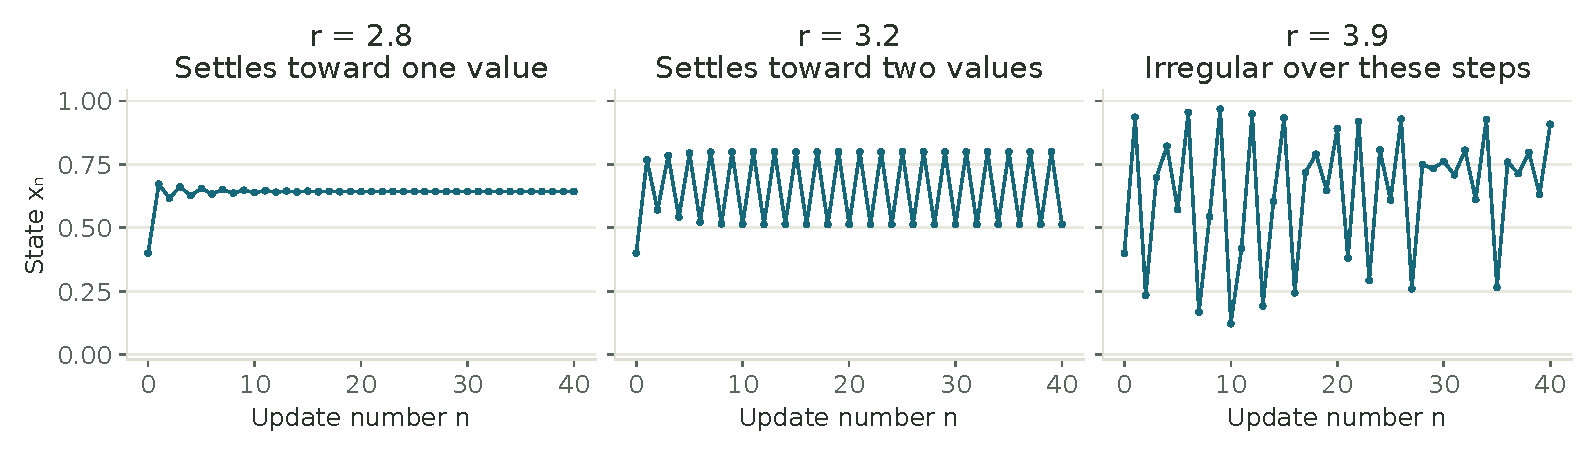
\includegraphics[width=\linewidth]{../assets/week10/logistic-behaviors.pdf}
\caption*{Each panel starts at x$_0$ = 0.4 and shows 40 updates. The parameter changes; the formula stays the same. A finite plot shows numerical behavior, not a proof about every future update.}
\end{figure}

{\small\renewcommand{\arraystretch}{1.35}\begin{tabularx}{\linewidth}{@{}YYY@{}}\toprule
Behavior & What to look for & Example\\
\midrule
Fixed point & Later values approach one state. & r = 2.8 approaches 1 $-$ 1/2.8 $\approx$ 0.642857.\\
Cycle & Later values approach a repeating pattern. & r = 3.2 approaches a two-cycle near 0.5130 and 0.7995.\\
Chaotic dynamics & Bounded irregular motion with sensitivity to nearby starts. & At r = 3.9, the nearby trajectories below separate substantially.\\
\bottomrule\end{tabularx}}





\begin{tcolorbox}[title={A larger r does not mean ``more chaos'' every time},breakable,colback=warm,colbacktitle=warm,coltitle=gold,colframe=gold!35]

There are periodic windows among the chaotic parameter ranges. For example, \(r=3.83\) has an attracting three-cycle. There are also exceptional starting values: at \(r=4\), the exact start \(x_0=0.5\) gives \(0.5\to1\to0\to0\). The explorer includes both examples.


\end{tcolorbox}


\begin{tcolorbox}[title={Pause and try 4},breakable]
With \(r=2.8\) and \(x_0=0.2\), calculate just the next state.
\end{tcolorbox}


\clearpage

\section{Knowing a rule and measuring a state are different tasks}

A deterministic rule repeats its result from exactly the same input. An observation usually leaves uncertainty about that input. Follow two plausible starts to see whether their forecasts remain close.


\begin{tcolorbox}[title={Example 6 \textperiodcentered{} A difference of one ten-thousandth},breakable]

Use \(r=3.9\) with \(x_0=0.4000\) and \(y_0=0.4001\). The first updates are

\[x_1=3.9(0.4)(0.6)=0.936,\qquad y_1=3.9(0.4001)(0.5999)=0.936077961.\]
The initial gap is 0.0001; after the first update it is about 0.000078. The gap \emph{shrinks initially}. Sensitivity does not require the gap to grow at every step.


\end{tcolorbox}


\begin{figure}[!htbp]
\centering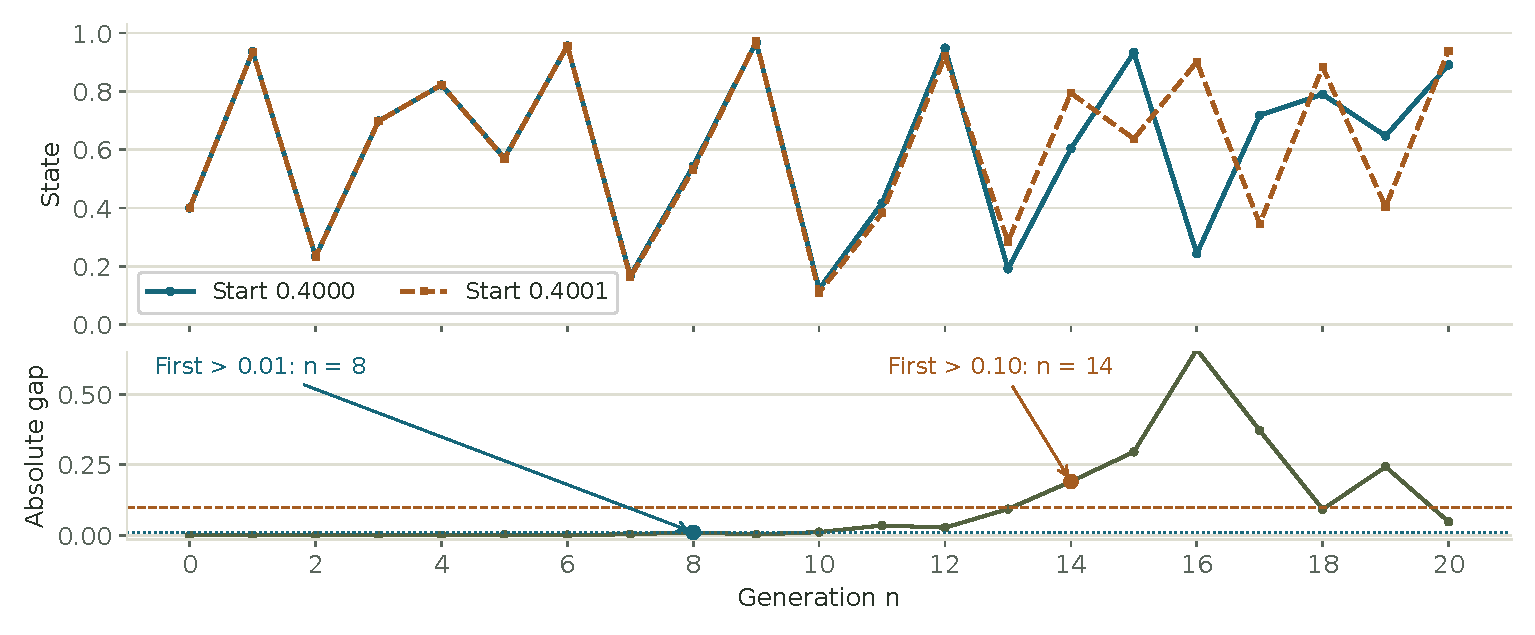
\includegraphics[width=.87\linewidth]{../assets/week10/forecast-sensitivity.pdf}
\caption*{The upper plot shows the states; the lower plot shows their absolute gap. Both calculations use full stored precision. Displayed decimals are rounded only for reading.}
\end{figure}


For this pair, the first gap above 0.01 occurs at generation 8; the first above 0.10 occurs at generation 14. A practical \emph{forecast horizon} depends on the initial uncertainty, the rule, and the decision tolerance.


Two trajectories illustrate sensitivity; they are not a confidence interval. A fuller uncertainty study would propagate many plausible starts or an appropriate uncertainty model.


\begin{tcolorbox}[title={Round for display, not between updates},breakable,colback=warm,colbacktitle=warm,coltitle=gold,colframe=gold!35]

Rounding 0.4001 to 0.400 makes the two starts identical. Premature rounding during iteration also changes later inputs. Keep the calculator's stored value and round only the reported numbers.


\end{tcolorbox}

\begin{tcolorbox}[title={Pause and try 5},breakable]
At generation 8, the gap is about 0.010896. At generation 9 it is about 0.003207. Has the first crossing of 0.01 moved to a later generation?
\end{tcolorbox}


\clearpage

\section{What does a shorter ruler reveal?}

A coarse map skips small bends in a boundary. A finer map follows more of them. The \emph{coastline paradox} asks what happens to a reported length as the observation scale changes.



\begin{figure}[!htbp]
\centering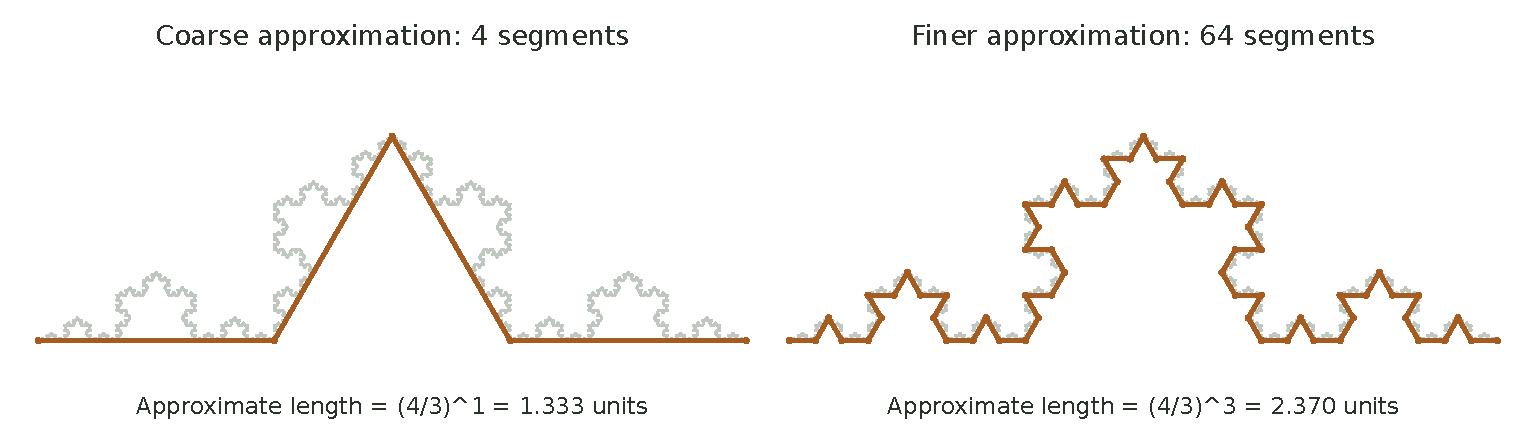
\includegraphics[width=\linewidth]{../assets/week10/scale-measurement.pdf}
\caption*{A schematic illustration, not field data. The gray boundary is the same in both panels. The colored measuring route changes with resolution.}
\end{figure}


\begin{tcolorbox}[title={Example 7 \textperiodcentered{} State both the length and the ruler},breakable]

In this invented survey, measured length equals ruler length times the number of placements.



{\small\renewcommand{\arraystretch}{1.35}\begin{tabularx}{\linewidth}{@{}YYYY@{}}\toprule
Ruler length & Placements & Measured length & In kilometers\\
\midrule
100 m & 80 & 100 $\times$ 80 = 8,000 m & 8.00 km\\
50 m & 200 & 50 $\times$ 200 = 10,000 m & 10.00 km\\
25 m & 520 & 25 $\times$ 520 = 13,000 m & 13.00 km\\
12.5 m & 1,340 & 12.5 $\times$ 1,340 = 16,750 m & 16.75 km\\
\bottomrule\end{tabularx}}


The measured coastline has not suddenly grown. The smaller ruler follows detail that the larger ruler skipped. A meaningful report includes the measurement scale and method.


\end{tcolorbox}

In an ideal Koch curve, finite-stage lengths grow without bound. Natural coastlines are physical objects, with tides, changing shorelines, and limits to how a boundary is defined and observed. Approximate fractal behavior across some scales does not establish literally infinite physical length.


\begin{tcolorbox}[title={Connection to optimization \textperiodcentered{} Does a complicated boundary change the method?},colback=warm,colbacktitle=warm,coltitle=gold,colframe=gold!35,breakable]

The corner-point method from Week 8 applies to a feasible polygon defined by linear inequalities. Replacing an edge with an irregular or fractal boundary changes the mathematical problem. A finite approximation may have many corners and may be nonconvex; the original list of vertices and linear constraints no longer describes it.


A bounded region can still have a finite, well-defined area even when its ideal boundary has infinite length. Infinite perimeter does not automatically imply undefined area. The chosen map resolution should match the decision we need to make.


\end{tcolorbox}


\begin{tcolorbox}[title={Pause and try 6},breakable]
A 20-meter ruler needs 600 placements. A 10-meter ruler needs 1,300 placements. Report both measured lengths.
\end{tcolorbox}


\clearpage

\section{What kind of question are we asking?}


{\small\renewcommand{\arraystretch}{1.35}\begin{tabularx}{\linewidth}{@{}YYY@{}}\toprule
Example & What we can calculate & What still needs care\\
\midrule
Collatz & The route, update count, and peak for a chosen start. & A finite collection of successes does not prove a universal claim.\\
Koch and Sierpinski & Exact finite-stage counts, lengths, and area fractions. & The drawn stage is finite; the ideal fractal is a limit.\\
Logistic map & The next state from an exact input; comparisons across starts. & Measurement uncertainty and sensitivity limit useful horizons.\\
Coastline & Length under a specified scale and method. & Different resolutions answer different measurement questions.\\
AI text generation & Probabilities in a model and the consequences of a chosen token. & A probable continuation is not evidence that its claim is true.\\
\bottomrule\end{tabularx}}


Across this course, mathematics has given us ways to represent quantities, describe data, compare choices, follow feedback, and trace networks. Here those tools meet a final habit: identify the rule, identify the observation, and state what your conclusion actually covers.


\subsection*{A final example: the output becomes the next input}
In autoregressive text generation, a chosen token is appended to the context before the next token is predicted. In this invented word-level model, an early choice changes the next distribution.
\begin{center}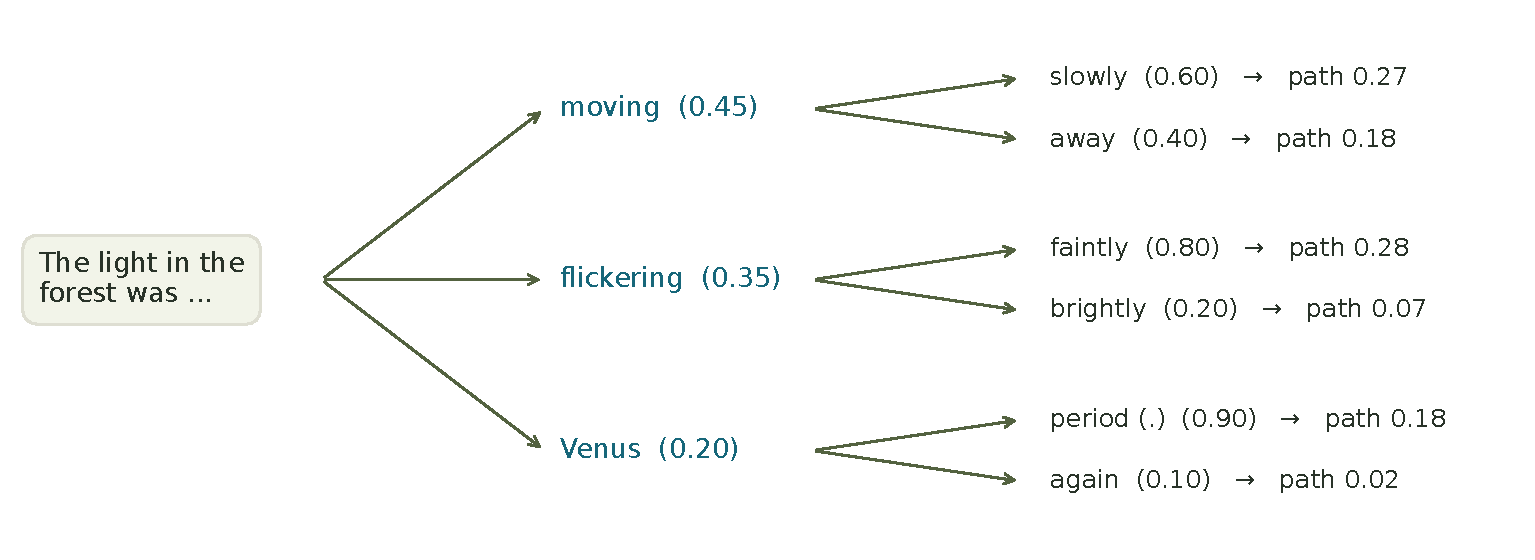
\includegraphics[width=.95\linewidth]{../assets/week10/ai-branches.pdf}\end{center}
The path ``moving then slowly'' has probability $0.45(0.60)=0.27$, while ``flickering then faintly'' has probability $0.35(0.80)=0.28$. The most probable first token need not begin the most probable whole path. Neither probability verifies what an actual light was doing.

\clearpage
\section*{Chapter Review}
\begin{enumerate}
\item Follow Collatz from 11. Record its update count and peak. If another trajectory later reaches 11, what happens to its remaining route?
\item At Koch stage 4, with an original segment of length 1, find the segment count, length per segment, and total length. How does the total change if the original length is 9 meters?
\item At Sierpinski stage 4, find the filled-triangle count and remaining area fraction. How can these move in different directions?
\item For $r=2.8$, start at 0.2. Calculate the first update and the nonzero fixed point. Why are they different quantities?
\item For $r=3.8$ with starts 0.40 and 0.41, calculate the first update at which the absolute gap exceeds 0.05. Retain full stored precision between updates.
\item In the $r=3.9$ example, let a model population be $N_n=100{,}000x_n$ fish. How many fish do the starting states 0.4000 and 0.4001 represent? At which generations does their gap first exceed 1,000 fish and 10,000 fish?
\item A 50-meter ruler requires 260 placements and a 25-meter ruler requires 580. Report both measured coastline lengths with their scales.
\item A computer verifies Collatz for every integer in a finite interval. What conclusion is justified? Give a family of infinitely many starting integers whose convergence can be proved directly.
\item In a toy AI model, $P(\text{moving})=0.45$ and $P(\text{slowly}\mid\text{moving})=0.60$, while $P(\text{flickering})=0.35$ and $P(\text{faintly}\mid\text{flickering})=0.80$. Compare the two path probabilities. Does either probability establish what an actual light in a forest was doing?
\end{enumerate}
\begin{tcolorbox}[title={A connection to optimization},breakable]
Begin with a rectangle 10 units wide and 5 units high, of area 50. Replace its top edge by outward-pointing Koch bumps. At stage 1, the added triangle has side $10/3$ and area $25\sqrt3/9\approx4.8113$. At stage 2, four triangles of side $10/9$ add $100\sqrt3/81\approx2.1383$. Thus the area is approximately 56.9496, while the perimeter is $20+10(4/3)^2\approx37.7778$.

At later stages, each added area is $4/9$ of the preceding addition, so their sum converges while the top-edge length diverges. Infinite ideal boundary length does not imply undefined area. Such a boundary also changes the feasible-set model; the original linear inequalities and corner list no longer describe it.
\end{tcolorbox}

\clearpage
\section*{Solutions and Further Reading}
{\small\setlength{\parskip}{3pt}\setlist{itemsep=2pt,topsep=2pt}

\paragraph{Check 1.} 
The values become 32 and 32.8. The absolute gap is 0.8. Relative to 32, the gap is \(0.8/32=0.025=2.5\%\), exactly the initial relative gap.


\paragraph{Check 2.} 
The conjecture holds for those 10,000 starting integers. The experiment provides evidence for the universal conjecture; it does not prove it for all positive integers.


\paragraph{Check 3.} 
Each segment has length \((1/3)^3=1/27\). There are 64 segments, so \(L_3=64/27\). The one-third factor is applied three times.


\paragraph{Check 4.} 
\(x_1=2.8(0.2)(0.8)=0.448\). It is not the fixed point; it is the first update from the chosen start.


\paragraph{Check 5.} 
No. The first crossing is still generation 8. The trajectories can later move closer again. ``First exceeds'' does not mean ``stays above forever.''


\paragraph{Check 6.} 
The coarse measurement is \(20\cdot600=12{,}000\) meters (12 km). The finer measurement is \(10\cdot1{,}300=13{,}000\) meters (13 km). Report the ruler sizes along with the lengths.


\subsection*{Review answers}
\begin{enumerate}
\item From 11: 14 updates, peak 52. Routes that reach 11 follow its future route.
\item $256$ segments, each of length $1/81$, total $256/81\approx3.1605$. From a 9-meter original, total length is $9(256/81)=256/9\approx28.4444$ meters.
\item $81$ triangles; area $81/256\approx0.3164$. Each new triangle has one-quarter its parent's area; the three remaining pieces together retain only three quarters.
\item First update $0.448$; nonzero fixed point $1-1/2.8\approx0.642857$. The first depends on the chosen start; the second is unchanged by the update.
\item Update 4, with gap approximately 0.078197. The preceding three gaps are about 0.007220, 0.022805, and 0.035779.
\item 40,000 and 40,010 fish; first gaps above 1,000 and 10,000 fish occur at generations 8 and 14. At generation 14, the gap is approximately 19,074 fish. The reference population is a scale chosen for this toy model, not a fitted carrying capacity for a real lake.
\item 13 km using the 50-meter ruler; 14.5 km using the 25-meter ruler.
\item The tested interval only. Every power of 2 reaches 1 by repeated halving.
\item $0.45(0.60)=0.27<0.35(0.80)=0.28$. Model continuation probabilities do not verify claims about the world.
\end{enumerate}
\subsection*{Further reading}
These sources provide background, not additional required assignments.
\begin{itemize}
\item R. M. May (1976), \emph{Simple mathematical models with very complicated dynamics}. \href{https://doi.org/10.1038/261459a0}{Nature 261, 459--467}.
\item R. De Leo and J. A. Yorke (2021), \emph{The graph of the logistic map is a tower}. \href{https://doi.org/10.3934/dcds.2021075}{DCDS 41, 5243--5269}.
\item A.-S. Elsenhans (2026), \href{https://www.antsxvii.org/papers/antsxvii-elsenhans-paper.pdf}{\emph{Numerical verification of the Collatz conjecture for billion digit random numbers}}.
\item B. Mandelbrot (1967), \emph{How long is the coast of Britain?} \href{https://doi.org/10.1126/science.156.3775.636}{Science 156, 636--638}.
\item A. Vaswani et al. (2017), \href{https://arxiv.org/abs/1706.03762}{\emph{Attention Is All You Need}}.
\end{itemize}
}
\end{document}
